% Nallino, Part I p. 59: Ptolemy's figure for the distance of the Sun, redrawn from the print: the circle
% of the Sun ABC (centre D), of the Moon EFG (centre H) and of the Earth KLM (centre N) on one axis, the
% cone of the rays ASC, the lines from N through the Moon to A and C, the diameter IPQ of the shadow and
% the line NQ that Nallino added. The circles and the lines are least-squares fits to the printed ink;
% the coordinates are PDF points of master page 148 less the origin (69.0, 127.0), y downward.
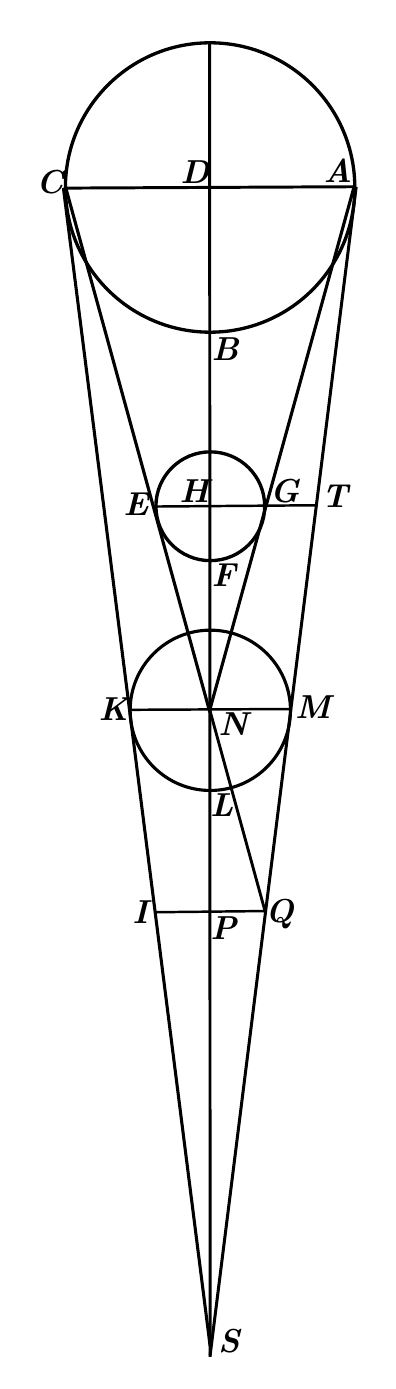
\begin{tikzpicture}[x=0.9916pt,y=-0.9916pt,line cap=butt,every node/.style={font=\fontsize{11.5}{11.5}\bfseries\itshape\selectfont,inner sep=0pt}]
\useasboundingbox (0,0) rectangle (124.00,486.00);
\draw[line width=1.20pt] (66.48,58.24) circle[radius=52.73];  % the circle of the Sun
\draw[line width=1.21pt] (66.55,174.40) circle[radius=19.82];  % the circle of the Moon
\draw[line width=1.13pt] (66.55,248.76) circle[radius=29.21];  % the circle of the Earth
\draw[line width=1.07pt] (66.31,5.51) -- (66.48,484.33);  % the axis, from the top of the circle of the Sun to S
\draw[line width=1.07pt] (13.75,58.46) -- (119.20,57.96);  % the diameter CA of the Sun
\draw[line width=1.11pt] (13.02,58.46) -- (66.48,480.40);  % C to S, touching the Earth at K
\draw[line width=1.09pt] (119.71,57.96) -- (66.48,483.84);  % A to S, touching the Earth at M
\draw[line width=1.13pt] (66.40,249.49) -- (13.75,57.91);  % N to C, touching the Moon at E
\draw[line width=1.13pt] (66.40,248.47) -- (119.19,57.11);  % N to A, touching the Moon at G
\draw[line width=0.89pt] (46.73,174.50) -- (105.20,174.04);  % the diameter EG of the Moon, drawn on to T
\draw[line width=0.89pt] (37.34,248.58) -- (95.76,248.29);  % the diameter KM of the Earth
\draw[line width=0.89pt] (46.46,322.34) -- (86.72,321.91);  % IPQ, the diameter of the shadow
\draw[line width=1.04pt] (66.40,248.77) -- (86.65,322.51);  % N to Q (added by Nallino)
\node at (8.12,56.11) {C};
\node at (60.95,52.78) {D};
\node at (112.97,52.33) {A};
\node at (72.02,117.13) {B};
\node at (39.44,173.65) {E};
\node at (60.68,168.79) {H};
\node at (93.71,168.70) {G};
\node at (111.98,170.77) {T};
\node at (71.39,199.48) {F};
\node at (31.25,248.17) {K};
\node at (74.90,253.75) {N};
\node at (103.97,247.63) {M};
\node at (70.67,283.45) {L};
\node at (40.97,322.15) {I};
\node at (71.30,328.27) {P};
\node at (91.82,323.05) {Q};
\node at (73.37,478.57) {S};
\end{tikzpicture}
